\section{Funzionamento}
Nella seguente sezione si descrive il funzionamento del veicolo, degli algoritmi utilizzati e delle scelte progettuali.

\subsection{Stack di guida autonoma}
La prima cosa da analizzare è il funzionamento dello stack di guida autonoma.
Lo stack funziona grazie a diversi processi, divisi (come descritto nell'introduzione) in perception, planning e control, di seguito una breve censita dei nodi ROS che permettono tale funzionamento:
Per quanto riguarda la parte di perception, vediamo due aspetti, i sensori e l'algoritmo di localizzazione:

\begin{itemize}
  \item \textbf{urg\_node}: È il nodo che permette di pubblicare sul topic ROS \textit{/scan} le pointcloud rilevate dal sensore Lidar, il tipo di dato utilizzato è chiamato \textit{LaserScan} e fornisce una serie di distanze che vanno insieme a formare ciò che il sensore Lidar rileva.
  \item \textbf{hunter\_ros2\_node}: Fornisce un interfaccia con il robot stesso, da questo nodo possiamo ricevere l'odometria calcolata a partire dal movimento delle ruote e, come vedremo successivamente, potremo pubblicare i comandi che il robot dovrà svolgere. Quello che interessa a noi al momento della perception è l'odometria del mezzo, che viene pubblicata sul tpoic \textit{/odometry} sottoforma di dato \textit{Odomentry}. 
  \item \textbf{particle\_filter}: Implementa l'algoritmo di localizzazione chiamato particle filter, questo algoritmo sfrutta per il suo funzionamento la mappa dell'ambiente in cui il robot si sta muovendo, l'odometria del veicolo e la pointcloud del sensore Lidar. Questo nodo pubblica la posizione calcolata sul topic ROS \textit{/pf/position} sottoforma di dato \textit{Odometry}.
\end{itemize}

\noindent Passando invece al momento del planning ci si avvale di due nodi:

\begin{itemize}
  \item \textbf{path\_logger}: Permette la registrazione di un percorso quando il veicolo viene guidato manualmentequesto percorso viene poi salvato in un file apposito.
  \item \textbf{path\_logger}: Questo nodo si occupa di pubblicare un percorso preregistrato o precalcolato da seguire, il dato è pubblicato sul topic \textit{/path}.  
\end{itemize}

\noindent Andiamo infine a descrivere il funzionamento della parte di controllo, questa è infatti composta da due nodi:

\begin{itemize}
  \item \textbf{purepursuit}: Si occupa di ricevere il percorso pubblicato sul topic \textit{/path} e a partire dalla posizione pubblicata dal nodo \textbf{particle\_filter} calcola i comandi da impartire al robot. I comandi vengono pubblicati sul topic\textit{/drive\_parameters} e sono di tipo \textit{Ackermann Stamped}, questo non è altro che un semplice tipo di messaggio ROS che incapsula il timestamp, un angolo di sterzo ed una velocità.
  \item \textbf{hunter\_ros2\_node}: Come descritto prima, questo nodo oltre a fornire l'odometria del mezzo, è anche capace di ricevere i comandi da impartire al robot. Il nodo è infatti in perenne ascolto sul topic \textit{/drive\_parameters} e ad ogni messaggio non farà altro che comunicare con l'interfaccia CAN del veicolo comunicandogli la velocità e l'angolo di sterzo da impostare.
\end{itemize}

\noindent di seguito uno schema riassuntivo di tutto il meccanismo:
\begin{figure}[h]
  \centering
  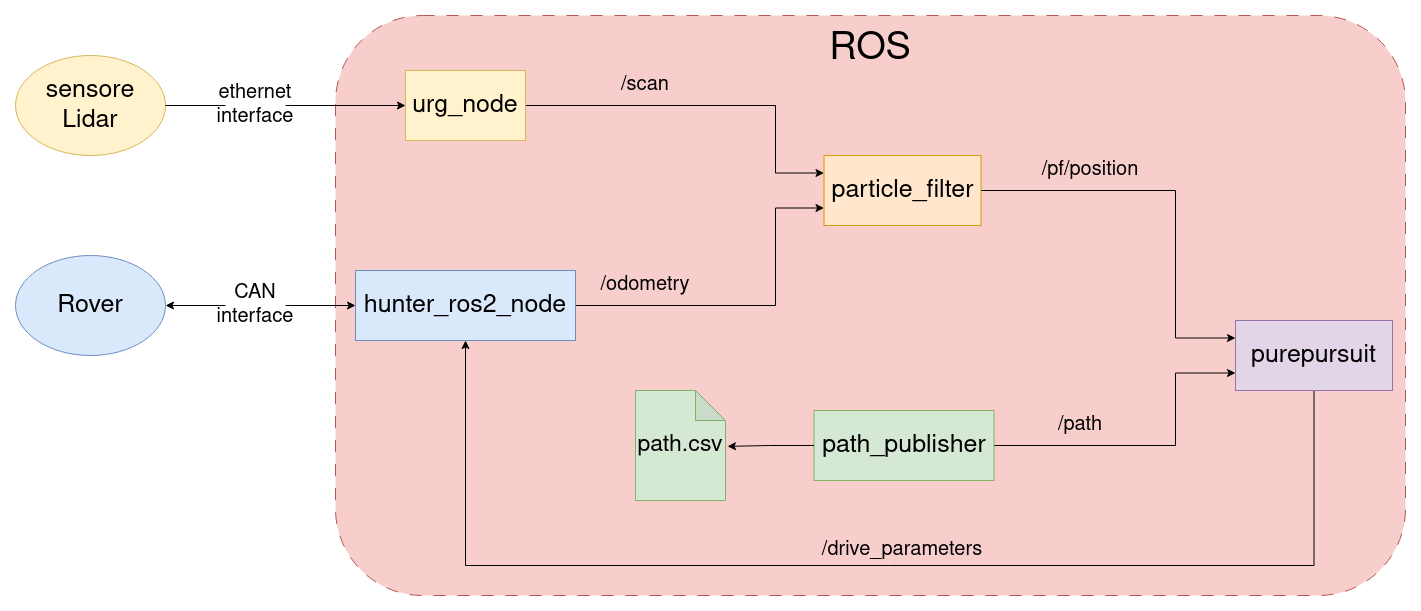
\includegraphics[width=1\textwidth]{figures/schema_guida_autonoma.png}
  \caption{Schema rissuntivo dello stack di guida autonoma}
  \label{Schema rissuntivo dello stack di guida autonoma}
\end{figure}

\subsection{guida remota}
Una volta illustrato e compreso il funzionamento dello stack di guida autonoma, è ora di passare alla pianificazione di quella remota.
La primissima domanda da porci è quale parte dello stack diventerà remoto, ad esempio si potrebbe decidere di svolgere solo la parte di planning da remoto e lasciare in resto in locale, o ad esempio di portare solo la perception. Si potrebbe anche decidere di far eseguire solo specifici nodi da remoto e lasciare in resto in locale.
\noindent Nella presente tesi si è scelto di portare in remoto quasi tutto lo stack, lasciando in locale solo i nodi che hanno strettamente bisogno dell'interfacciamento con l'hardare.

\noindent Nello specifico gli unici nodi che rimarranno in locale saranno:

\begin{itemize}
  \item \textbf{urg\_node}: Che sarà necessario per ricavare i dati dal sensore Lidar
  \item \textbf{hunter\_ros2\_node}: Necessario per ricavare l'odometria del mezzo e per inviare i comandi all'interfaccia CAN
\end{itemize}

\noindent Tutto il resto sarà gestito da remoto. Questo ci permette di poter scegliere con più flessibilità in quale modo pilotare il rover, si potrà infatti decidere sia di eseguire l'intero stack, senza modifiche, sulla macchina in remoto e di conseguenza inviare i comandi calcolati al mezzo, sia di poter guidare il veicolo completamente in manuale da un apposito operatore e di inviare solo i comandi scelti da quest'ultimo al veicolo.
